
\section{The iron-pnictides}

One of the most important recent breakthroughs in the field of high-$T_c$ superconductivity has been the discovery of the iron-pnictide superconductors in 2006~\cite{Kamihara2006, Kamihara2008} which sparked an enormous amount of interest when it was discovered that they could be tuned to transition temperatures above the historic limit in Nb$_3$Ge of \unit{23}{\kelvin}~\cite{Attfield2010}.

Since their initial discovery, many different superconductors have been discovered which all feature similar tetrahedrally bonded transition metal-pnictide or transition metal-chalcogenide\footnote{For convenience, when referring to iron-pnictides in this thesis, unless otherwise stated, it should be taken to also include the various transition metal-pnictide/chalcogenide combinations that feature this tetrahedral structure.} layers which are grouped by structure into families as shown in figure~\ref{Fig:Intro:PnictideUnitCells}.
\begin{figure}[htbp]
    \begin{center}
        \includegraphics[scale=1.1]{Chapter-Introduction/Figures/PnictideUnitCells/PnictideUnitCells}
        \caption{From left to right: 1111 unit cell, 122 unit cell, 111 unit cell, 11 unit cell. Adapted from ref.~\cite{Johnston2010}.}
        \label{Fig:Intro:PnictideUnitCells}
    \end{center}
\end{figure}
The families are labelled according to the ratios of the constituent elements, so for example the `1111' family features four element types in equal proportion, the `122' family features three element types with one of the elements being half as abundant as the other two. In the case of a doped or substituted material, this labelling refers to the stoichiometric parent compound. 

With the exception of the 11 family, the `iron-pnictide' layers are separated by the so called `charge reservoir' layers, which are comprised of a single element type in the case of the `122' and the `111' families and two element types in the `1111' family as shown in figure~\ref{Fig:Intro:PnictideUnitCells}.

Although the highest $T_c$ values have been attained with compounds in the `1111' family (SmFeAsO$_{1-x}$F$_x$ has a $T_c$ of \unit{55}{\kelvin}~\cite{Ren2008}, Gd$_0.8$Th$_{0.2}$FeAsO has a $T_c$ of \unit{56}{\kelvin}~\cite{Wang2008} and Sr$_{1-x}$Sm$_x$FFeAs has a $T_c$ of \unit{56}{\kelvin}~\cite{Wu2009}), it is comparatively difficult to grow large single crystals of the 1111 family causing the emphasis to be shifted to the 11 and the 122 families, especially for neutron scattering studies~\cite{Johnston2010}.

The most studied materials with these transition metal-pnictide/chalcogenide layers typically feature As and P in the pnictide case and Se and Te in the chalcogenide case with the highest $T_c$ values being attained with Fe as the transition metal although superconductivity has been achieved with stoichiometric compounds featuring Ru, Rh, Ir and Ni as the transition metal~\cite{Johnston2010}.



\subsection{Fermiology of the pnictides}

The Fermiology --- i.e. the nature of the Fermi surface --- is key to the formation of the \ac{SDW} state, the onset of which provides the fluctuations necessary for spin-fluctuation mediated pairing and will be described in more detail in the next section. The Bristol group has published a series of results on the Fermiology of various iron-pnictides obtained by \acf{dHvA} measurements which compliment measurements of the Fermi surface by other groups using \acf{ARPES}. A summary of some of these measurements are detailed below.

LaFePO, a member of the 1111 family, has a relatively low superconducting transition temperature of \unit{$\sim$6}{\kelvin}, nonetheless it is a good example to demonstrate the quasi-cylindrical electron and hole Fermi surfaces typical to the iron-pnictides. Figure~\ref{Fig:Intro:PnictideFS} shows the Fermi surface from \acf{DFT} calculations using \ac{GGA} with hole pockets centred around $\Gamma$ and the electron pockets centred around $M$ (adapted from ref.~\cite{Carrington2009}).

The momentum separated hole and electron pockets are indicative of a semi-metal, which distinguishes the pnictides from the cuprates\footnote{Cuprates are the other major class of high-$T_c$ superconductors, see section~\ref{Sec:Intro:PhaseDiagram} for an introduction.} which are charge insulating antiferromagnets in the undoped state. 

The top right two panels of figure~\ref{Fig:Intro:PnictideFS} shows slices along the 110 plane through the LaFePO \ac{BZ} which demonstrate how the mean field \ac{DFT} calculations had to be adjusted by uniformly shifting the energies in each of the bands to match the \ac{dHvA} measurements. This leads to smaller Fermi surface volumes than the unadjusted \ac{GGA} calculations.

The LaFePO Fermi surfaces are quasi-2D with only relatively weak energy dispersions in $k_z$ which are more pronounced for the electron pockets. In contrast, the middle portion of figure~\ref{Fig:Intro:PnictideFS} shows the Fermi surface for the non-superconducting 122 family iron-pnictide CaFe$_2$P$_2$ measured by the Bristol group~\cite{Coldea2009}. This also demonstrates semi-metal characteristics but a much stronger $k_z$ dispersion leading to entirely 3D hole surfaces. In this case the \ac{GGA} calculations matched the measured \ac{dHvA} data closely with no energy shifts required.
\begin{figure}[htbp]
    \begin{center}
        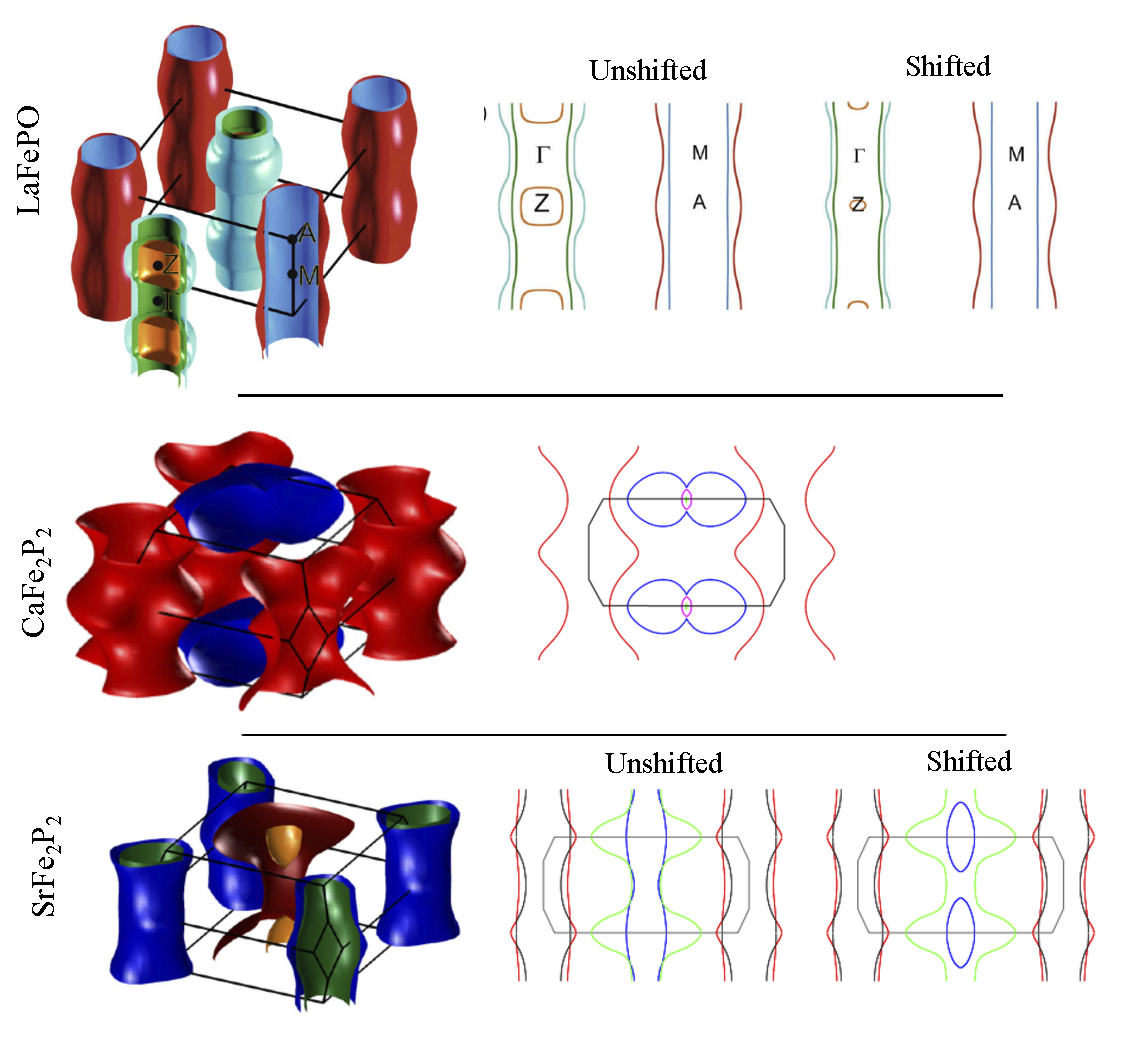
\includegraphics[scale=0.7]{Chapter-Introduction/Figures/PnictideFS/PnictideFS}
        \caption{Fermi surfaces of various iron-pnictides from top to bottom: LaFePO (top) with 110 slices of the \ac{BZ} showing the \ac{DFT} calculations both before (unshifted) and after (shifted) adjustments to match the \ac{dHvA} data. CaFe$_2$P$_2$ (middle) with a 110 slice across the Fermi surface. \SrFeP{} (bottom) with 110 slices similar to LaFePO. Adapted from refs.~\cite{Carrington2009, Coldea2009, Carrington2011, Analytis2009}.}
        \label{Fig:Intro:PnictideFS}
    \end{center}
\end{figure}

Comprehensive determination of the Fermi surface of Sr$_2$P$_2$, another non-superconducting 122 phosphide, also shows 3D hole Fermi surfaces as demonstrated in the bottom row of figure~\ref{Fig:Intro:PnictideFS}. In this case it was necessary to shift some of the bands from the \ac{GGA} calculations to match the \ac{dHvA} data. Here the outer hole pocket is strongly warped along $k_z$ but does not pinch off as in the CaFe$_2$P$_2$ case, the inner hole pocket after the shift becomes pinched off and fully 3D.

\SrFeP, CaFe$_2$P$_2$ as well as \BaFeP{} form the end members of superconducting series that begin with the arsenide counterparts. The arsenide parent compound change from the tetragonal structure to an orthorhombic structure below a characteristic temperature, $T_s$ which occurs close to a transition from a paramagnetic phase to a stripe \ac{SDW} state below the N\'eel temperature, $T_N$. This affects the Fermiology by a doubling of the real-space unit cell volume and therefore halving of the \ac{BZ} volume.
\begin{figure}[htbp]
    \begin{center}
        \includegraphics[scale=0.7]{Chapter-Introduction/Figures/AsReconstruction/AsReconstruction}
        \caption{(a) Illustrative 2D projection of the Fermi surface of the tetragonal \ac{BZ} (solid line) with the reconstructed \ac{BZ} as a dashed line (b) Schematic semi-metal band structure of the tetragonal phase showing the hole band at $\Gamma$ and the electron band at $M$ with the dashed lines showing how the folding of the \ac{BZ} aligns the hole bands onto the electron bands (c) The folded \ac{SDW} \ac{BZ} with the resulting gap at the Fermi energy.}
        \label{Fig:Intro:AsReconstruction}
    \end{center}
\end{figure}
The halving of the \ac{BZ} `folds' the larger zone along the dashed lines illustrated in figure~\ref{Fig:Intro:AsReconstruction}~(a) causing the electron bands in the tetragonal \ac{BZ} corners to be superimposed on the hole bands around $\Gamma$ at the \ac{BZ} centre. Figure~\ref{Fig:Intro:AsReconstruction}~(c) demonstrates how the overlaying of the hole and electron bands in momentum space opens a gap around the Fermi energy and the Fermi surface disappears. In practice, the hole and electron Fermi surfaces are not sufficiently symmetric to perfectly cancel and so several small residual hole and electron pockets are left over. \acs{LDA}+U calculations and \ac{dHvA} measurements were performed on BaFe$_2$As$_2$~\cite{Analytis2010b} with the Fermi surface from this publication reproduced in figure~\ref{Fig:Intro:FSBaFeAs}.
\begin{figure}[htbp]
    \begin{center}
        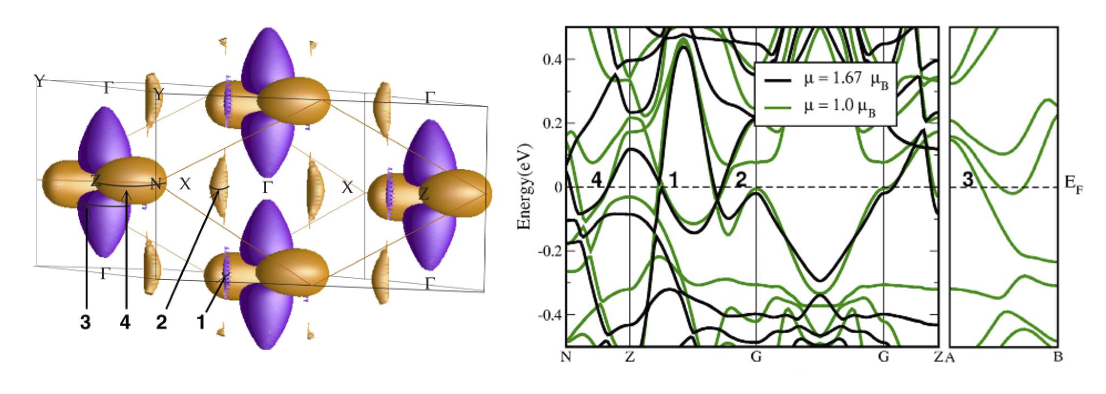
\includegraphics[scale=0.7]{Chapter-Introduction/Figures/FSBaFeAs/FSBaFeAs}
        \caption{Left: BaFe$_2$As$_2$ Fermi surface from \acs{LDA}+U calculations adjusted to fit \ac{dHvA} measurements. Right: Corresponding band structure showing both with (green) and without (black) corrections to $U$.}
        \label{Fig:Intro:FSBaFeAs}
    \end{center}
\end{figure}
Similar measurements were also performed on detwinned\footnote{Similar $a$ and $b$ lattice vectors in orthorhombic crystals can lead to imperfections where one region is rotated by \unit{90}{\degree} with respect to another region. This is known as twinning and when a material which is susceptible to twinning has all the $a$ and $b$ axes aligned, the crystal is said to be `detwinned'.} samples of BaFe$_2$As$_2$ by Terashima \etal~\cite{Terashima2011} which demonstrated similar small pockets with only small difference in detail.


\subsection{The \BaFeAsP{} series}


The \BaFeAsP{} series is one of many that stem from the parent compound \BaFeAs, although unlike the electron doped \BaCoFeAs{} and the hole doped \BaKFeAs{} series, the \BaFeAsP{} progression is entirely isovalent meaning that the changes affected due to the P substitution are due to structure and chemical pressure rather than additional charge carriers. Nonetheless, superconductivity occurs with a very similar phase diagram as with the charge-doped examples in the same $122$ family of iron-pnictide materials.\footnote{See for example figure~1 in ref.~\cite{Paglione2010}.}. 

At $x=0$ the \BaFeAsP{} series begins at \BaFeAs, a compound which becomes antiferromagnetic at around \unit{138}{\kelvin}, and moves with increasing $x$ towards \BaFeP{} which is metallic to low temperatures. Neither end members are superconducting, however as As is substituted for P, the low temperature antiferromagnetic state decays, giving way to superconductivity which kicks in at approximately $x=0.18$ and increases to the optimal substitution of $x=0.31$. Superconductivity then decreases until it gives way to a paramagnetic ground state at around $x=0.71$. Figure~\ref{Fig:Intro:PhaseDiagram} shows the phase diagram adapted from ref.~\cite{Nakai2010a} as determined by resistivity measurements. 
\begin{figure}[htbp]
    \begin{center}
        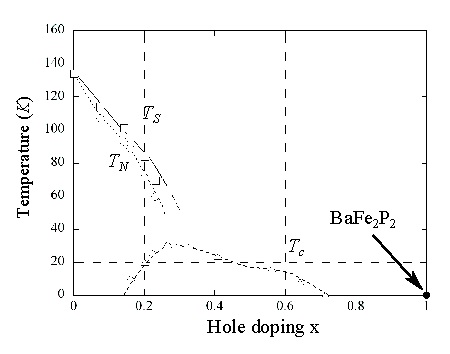
\includegraphics[scale=1.0]{Chapter-Introduction/Figures/PhaseDiagram/PhaseDiagram}
        \caption{Phase diagram adapted from ref \cite{Nakai2010a} measured by resistivity. $T_s$, $T_N$ and $T_c$ are the structural transition, the antiferromagnetic transition and the superconducting transition temperatures respectively.}
        \label{Fig:Intro:PhaseDiagram}
    \end{center}
\end{figure}
Also detailed in the phase diagram is the structural transition which occurs as the tetragonal $I4/mmm$ cell moves to an orthorhombic cell as it passes below the line marked $T_s$. This coincides with the reconstruction of the Fermi surface detailed in the previous section.

 The progression along the series is isovalent since P and As are in the same periodic group -- group $V$. The net effect of the substitution is to apply an increasing chemical pressure as $x$ moves towards $1$. Several reports show that applying high \emph{physical} pressure ($\sim$\unit{5}{\giga\pascal}) to \BaFeAs{} results in a similar phase diagram with an antiferromagnetic phase and superconductivity up to $\sim$\unit{30}{\kelvin}~\cite{Yamazaki2010,Colombier2009,Alireza2009} with Klintberg \etal~\cite{Klintberg2010} presenting a direct comparison between the two types of pressure. As pressure is applied, the unit cell $a$ axis shrinks slightly less than the $c$ axis ($\sim3\%$ cf. $\sim4.5\%$ respectively). Interestingly the $c$ axis shrinking largely occurs in the Fe-Pnictide plane leading to some theories of the superconductivity emerging from the tetrahedral bond angle between the Fe and the pnictogen.
\begin{figure}[htbp]
    \begin{center}
        \includegraphics[scale=1.0]{Chapter-Introduction/Figures/UnitCell/UnitCell}
        \caption{The tetragonal unit cell of the 122 \BaFeAsP{} series clearly showing the tetragonally bonded Fe(As,P) layers.}
        \label{Fig:Intro:UnitCell}
    \end{center}
\end{figure}


The Fermiology of the \BaFeAsP{} series from a substitution of $x=0.41$--$1.0$ has been previously measured by members of the group at Bristol using dHvA oscillations~\cite{Shishido2010}. As suggested in the Shishido reference~\cite{Shishido2010}, since dHvA has been observed across such a large range of substitutions, it implies that the material is not prone to disorder as is the case in many charge doped series~\cite{VanderBeek2010} making the series an excellent candidate for dHvA studies. This could be explained by the fact that the substitution is isovalent and that there is relatively little contribution at the Fermi surface from the pnictide sites\footnote{See for example, the orbital character for the iron sites from \ac{DFT} calculations presented in figure~\ref{Fig:ResD:Band2DCharacterVsKz} in chapter~\ref{Sec:ResD}.} where the substitution takes place, meaning the Fermi surface should not be strongly disrupted when traversing the series. The Fermi surfaces from the Shishido paper have been characterised for x ranging from $0.41$ to $1$ for electron sheets only but have clearly shown that the DFT calculations consistently overestimate the size of the surfaces. They also show a linear progression of the electron orbit sizes which is proportional to $x$. Moreover, dHvA measurements on the material with $x=0.63$ have been performed where one of the hole surface extrema was observed~\cite{Analytis2010c} however DFT calculations as well as comparisons with \SrFeP~\cite{Analytis2009} give evidence for a second hole Fermi surface for materials towards the P end of the series, (towards the As end of the series, there appears this second hole and a \emph{third} hole surface similar but smaller to the other hole sheets). If the electron Fermi surfaces are oversized in the DFT calculations, then the hole Fermi surface volumes should also be oversized in order to remain compensated (electrically neutral). What is not clear though is whether the \emph{shapes} of the hole pockets are also altered in the compounds leading to \BaFeP. DFT calculations show the larger of the hole pockets in particular undergoing significant geometric changes, specifically in that it becomes much more three dimensional as P substitution becomes more complete. The Fermi surface of the opposite end-member, \BaFeAs, has been fully characterised by previous \ac{ARPES} measurements~\cite{Kondo2010a} and dHvA~\cite{Terashima2011, Analytis2010b}. Intermediate unreconstructed superconducting compounds have been partially characterised by \ac{dHvA}~\cite{Analytis2010c} and \ac{ARPES}~\cite{Yoshida2010}. Coupled with a full characterisation of the Fermiology of \BaFeP, this unreconstructed Fermi surface data can be used to interpolate Fermiology of the hole pockets across the portion of the phase diagram outside of the \ac{SDW} state.

The \ac{ARPES} measurements of the Fermi surface of \BaFeAs{} below the N\'eel temperature concluded that despite some $k_z$ dispersion in the Fermi surfaces, there is adequate nesting to form the antiferromagnetic state. Ab-initio DFT calculations~\cite{Shishido2010} of the paramagnetic state have shown the $k_z$ dispersion increasing with increasing P, with the outer hole pockets becoming more three-dimensional through the progression providing the partial nesting conditions necessary for pair forming \ac{SDW} fluctuations described in section~\ref{Sec:Intro:Nesting}\footnote{These calculations do not take into account the reconstruction below $T_s$ however for low $x$, and instead assume a hypothetical non-magnetic order.}



